\section{Anforderungsanalyse und Konzept}\label{sec:07_03_anforderungen_konzept}

Die allgemeinen Anforderungen ergeben sich aus der Aufgabenstellung:
\begin{itemize}
	\item Ermittlung von Stimmungsmachern im Bundestag
	\item Mathematische Analysen bezüglich der Sentiments im Bundestag
\end{itemize}

Zur Identifikation detaillierter Anforderungen fand im frühen Projektverlauf eine Absprache mit Gruppe 8 statt, welche die Benutzeroberfläche entwickelt.
Im Rahmen dieses Meetings wurde festgelegt, dass folgende Funktionalitäten notwendig sind:
\begin{itemize}
	\item Abfrage von Stammdaten:
	\begin{itemize}
		\item Sitzungen
		\item Fraktionen
		\item Abgeordnete
	\end{itemize}
	\item Abfrage des Graphen für Fraktionen und Abgeordnete. Die Übertragung des Graphen erfolgt durch gleichzeitige Übertragung der beteiligten Knoten (Abgeordnete bzw. Fraktionen) und der Nachrichten, die zwischen diesen verschickt wurden. Dabei werden Nachrichten zwischen zwei beteiligten Knoten aggregiert, um die übertragene Datenmenge zu reduzieren.
	\item Mathematische Analysen bezüglich des Sentiments im Bundestag. Als Ziel wurde die Darstellung von Boxplots angegeben. Daher wurde festgelegt, dass Minimum, unteres Quartil, Median, oberes Quartil und Maximum berechnet werden. Zum Vergleich der Sentiments innerhalb verschiedener Sitzungen soll die Möglichkeit der Filterung nach Sitzung vorgesehen werden.
\end{itemize}

\newpage
\subsection{Architektur}
Der zentrale Bestandteil des Teilprojekts Graphauswertung ist die Backend Applikation. Hier werden die Daten, die zuvor über die Datenbankmanager aus den Neo4j Datenbanken von Gruppe 4 und 5 gezogen werden, zusammengeführt und weiter verarbeitet. Die Daten werden unter anderem zu statistischen Kennzahlen aufbereitet und mittels des PageRank und Reverse PageRank analysiert. Anschließend werden diese Daten über HTTP-Schnittstellen für die Benutzeroberfläche zur Verfügung gestellt.
\begin{figure}[H]
	\centering
	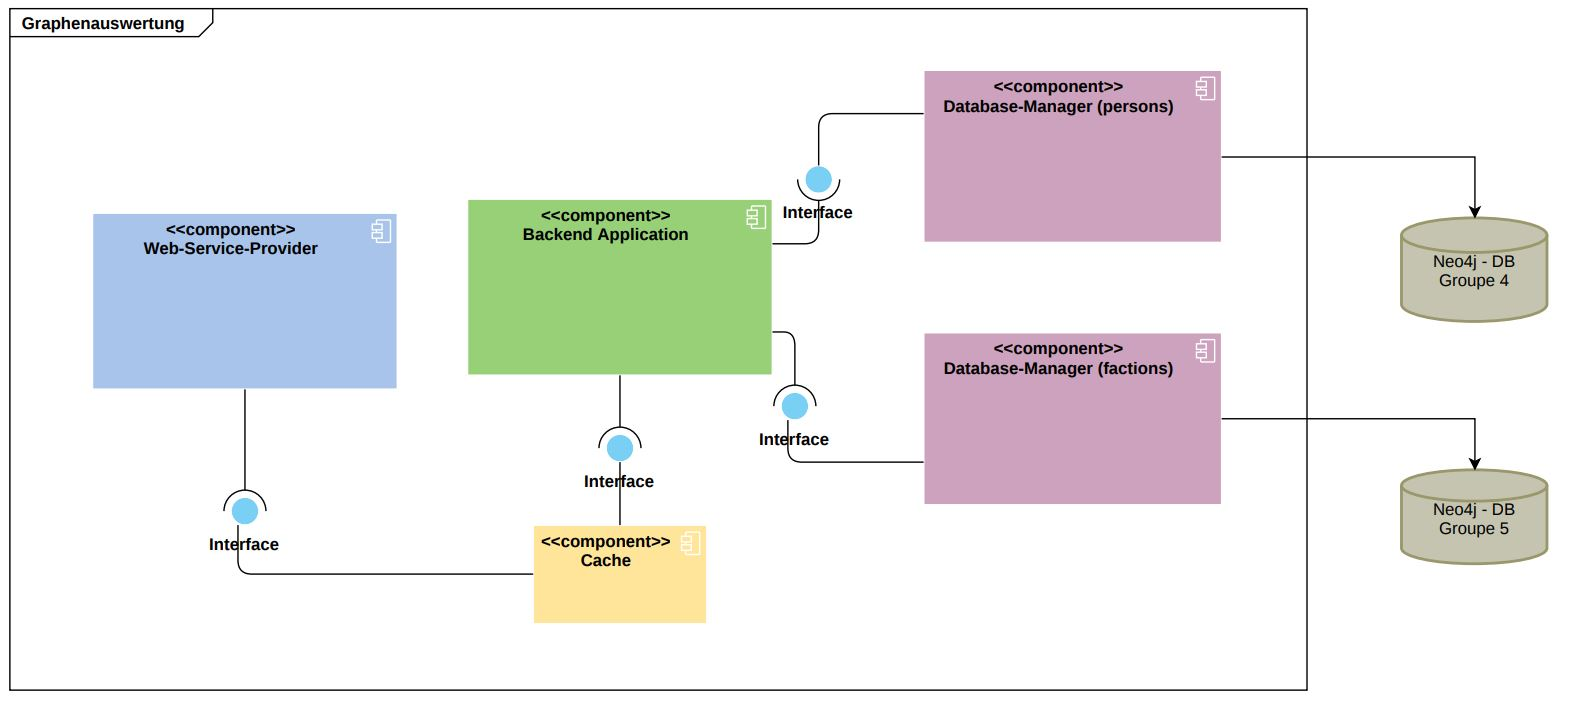
\includegraphics[width=450px, keepaspectratio]{images/07-Graphauswertung/graphenauswertung_architektur}
	\caption{Graphauswertung - Komponentendiagramm,\\Quelle: Eigene Darstellung, Tool: \cite{visual_paradigm}}
\end{figure}
\subsection{Schnittstellen}
Im Folgenden werden die HTTP-Schnittstellen zu dem angrenzenden Teilprojekt (Benutzeroberfläche) beschrieben und an einigen Beispielen erklärt, welche Daten dabei bereitgestellt werden. Als vorletztes Teilprojekt in der Datenkette wird als Backend für die Benutzeroberfläche agiert. Dabei werden die Daten aus den Neo4j Datenbanken herausgezogen, aufbereitet und über HTTP-Endpunkte dem Frontend in verschiedener Form zur Verfügung gestellt. Die gesamte Dokumentation und Beispielausgaben der Endpunkte sind in der README im GitHub-Repository \textit{Sentiments-of-Bundestag/Graphenauswertung}~\cite{github_endpoints} zu finden.
\\~\\
Die HTTP Schnittstellen wurden mithilfe des Microframework Python Flask \cite{flask} umgesetzt. Alle verfügbaren Endpunkte sind über GET erreichbar. Einige Endpunkte bieten mittels beigefügter Parameter Filtermöglichkeiten an. 
\begin{table}[ht]
	\caption{Abfrageparameter}
	\label{tab:filter}
	\begin{tabular}{|p{3 cm}|p{8.5 cm}|p{2.5 cm}|}
		\hline
		\textbf{Name} & \textbf{Beschreibung} & \textbf{Erwarteter Wert} \\
		\hline
		filter & Filtert die Nachrichten nach dem gegebenen Sentiment Typen. & POSITIVE, NEGATIVE \\
		\hline
		session & Filtert die Nachrichten nach der gegebenen Parlamentssitzungen. & sessionId aus \texttt{/sessions} \\
		\hline
		person & Filtert die Nachrichten nach den gegebenen Abgeordneten. & speakerId aus \texttt{/persons} \\
		\hline
		excludeApplause & Filtert alle Nachrichten aus, die mit \texttt{applause} markiert sind. & true \\
		\hline
		reverse & Wendet für die PageRank-Analyse den Reverse PageRank an. & true \\
		\hline
	\end{tabular}
\end{table} 
~\\
\textbf{\underline{Sessions:}}\newline
Der Endpunkt \textbf{\texttt{/sessions}} gibt eine Liste aller verfügbaren Parlamentssitzungen zurück.
\begin{lstlisting}
		[
			{
			 "sessionId": 138, 
			 "legislativePeriod": 19, 
			 "endDateTime": "2019-12-20T15:39:00+00:00", 
			 "startDateTime": "2019-12-20T09:00:00+00:00"
			},
			...
		]
\end{lstlisting}	
~\\	
\textbf{\underline{Factions:}} 
\newline
Der Endpunkt \textbf{\texttt{/factions}} gibt eine Liste aller Fraktionen zurück. Die Werte in \texttt{sessionIds} stehen für die Parlamentssitzungen, in denen Nachrichten mit anderen Fraktionen oder Abgeordneten ausgetauscht worden sind.
\newpage
~\\		
\textbf{\underline{Factions graph:}} \newline
Der Endpunkt \textbf{\texttt{/factions/graph}} gibt den Fraktionsgraphen basierend auf den Graphen der Datenbank von Gruppe 5 zurück. Die Nachrichten sind bereits aggregiert, also steht jede Verbindung zwischen Sender und Empfänger für alle Nachrichten in die jeweilige Richtung. Der Wert \texttt{count} ist die Anzahl aller für den aggregierten Eintrag berücksichtigten Nachrichten. Der Wert \texttt{sentiment} ist der Durchschnitt aller Sentiments aus den - für diesen aggregierten Eintrag berücksichtigten - Nachrichten. Der Durchschnitt ist zusätzlich durch die Fraktionsgröße gewichtet. Diese Schnittstelle bietet die Filteroptionen: person, session, excludeApplause, POSITIVE und NEGATIVE.	
\begin{lstlisting}
		{
			"factions": [
			 {
			  "name": "CDU/CSU",
			  "size": 246, 
			  "factionId": "F000"
			 },
			 {
			  "name": "SPD",
			  "size": 152,
			  "factionId": "F001"
			 }
			],
			"messages": [
			 {
			  "recipient": "F001",
			  "sender": "F000",
			  "sentiment": -1.399999976158142,
			  "count": 10,
			  "sessionIds": [46, 100]
			 },
			 {
			  "recipient": "F000",
			  "sender": "F001",
			  "sentiment": 0.1,
			  "count": 2,
			  "sessionIds": [46, 100]
			 }
			]
		}
\end{lstlisting}
\newpage
~\\	
\textbf{\underline{Persons:}}\newline
Der Endpunkt \textbf{\texttt{/persons}} gibt eine Liste aller Abgeordneten zurück. Diese Schnittstelle bietet die Filteroptionen: person, session, POSITIVE und NEGATIVE.
\begin{lstlisting}
[
    {
    "faction": "CDU/CSU",
    "factionId": "F000", 
    "name": "Frank Heinrich", 
    "role": "Platzhalter", 
    "speakerId": "MDB-24aa7763-e95d-4d1d-834c-de3cae2406d7",
    "sessionIds": [ 46, 100 ]
}, 
...
]
\end{lstlisting}
~\\
\textbf{\underline{Messages:}}\newline
Der Endpunkt \textbf{\texttt{/persons/messages}} gibt eine Liste aller Nachrichten zurück. Die Nachrichten sind nicht aggregiert. Diese Schnittstelle bietet die Filteroptionen: session, person, excludeApplause, POSITIVE und NEGATIV.	
\\~\\
\textbf{\underline{Persons graph:}}\newline
Der Endpunkt \textbf{\texttt{/persons/graph}} gibt den Abgeordnetengraphen, basierend auf den Graphen der Datenbank von Gruppe 4 zurück. 
Die Nachrichten sind bereits aggregiert, also steht jede Verbindung zwischen Sender und Empfänger für alle Nachrichten in die jeweilige Richtung. Der Wert \texttt{count} ist die Anzahl aller für den aggregierten Eintrag berücksichtigten Nachrichten. Der Wert \texttt{sentiment} ist der Mittelwert aller Sentiments aus den - für diesen aggregierten Eintrag berücksichtigten - Nachrichten. Diese Schnittstelle bietet die Filteroptionen: person, session, excludeApplause, POSITIVE und NEGATIVE.	
\\~\\
\textbf{\underline{Factions ranked:}}\newline
Der Endpunkt \textbf{\texttt{/factions/ranked}} gibt eine Liste aller Fraktionen, geordnet nach dem PageRank zurück. Diese Schnittstelle bietet die Filteroptionen: reverse, session, excludeApplause, POSITIVE und NEGATIVE.
\\~\\
\textbf{\underline{Persons ranked:}}\newline
Der Endpunkt \textbf{\texttt{/persons/ranked}} gibt eine Liste aller Abgeordneten, geordnet nach dem PageRank zurück. Diese Schnittstelle bietet die Filteroptionen: reverse, session, excludeApplause, POSITIVE und NEGATIVE.
~\\
\begin{lstlisting}
		[
			{
			 "faction": "DIE LINKE",
			 "factionId": "F003", 
			 "name": "Caren Lay", 
			 "rank": 0.029715244473085708, 
			 "role": "Platzhalter",
			 "sessionIds": [ 46, 100 ],
			 "speakerId": "MDB-c3f825cc-9b63-4241-85f9-df425f0c6486"
			}, 
			{
			 "faction": "CDU/CSU",    
			 "factionId": "F000",
			 "name": "Wolfgang Schaeuble", 
			 "rank": 0.029176551464191278, 
			 "role": "Platzhalter",   
			 "sessionIds": [ 46   ], 
			 "speakerId": "MDB-fd366231-9c25-416b-8604-e934d956e177"
			}
		]
\end{lstlisting}
~\\	
\textbf{\underline{Factions proportions:}}\newline
Der Endpunkt \textbf{\texttt{/factions/proportions}} gibt eine Liste aller Fraktionen mit dem jeweiligem Redeanteilen als Prozentwert zurück. Diese Schnittstelle bietet die Filteroptionen: session und excludeApplause.
\\~\\	
\textbf{\underline{Factions sentiment key figures:}} \newline
Der Endpunkt \textbf{\texttt{factions/sentiment/keyfigures}} gibt den Sentimentwert aller Fraktionen verrechnet in statistische Kennzahlen zurück. Diese Schnittstelle bietet die Filteroptionen: session und excludeApplause.	
\begin{lstlisting}
	{
	 "highest_sentiment": 16.04166666790843, 
	 "lowest_sentiment": 0.5, 
	 "sentiment_lower_quartile": 1.0, 
	 "sentiment_median": 2.5903602056205273, 
	 "sentiment_upper_quartile": 5.3949188850820065
	}
\end{lstlisting}	
\textbf{\underline{Persons sentiment key figures:}} \newline
Der Endpunkt \textbf{\texttt{persons/sentiment/keyfigures}} gibt den Sentimentwert aller Abgeordneten verrechnet in statistische Kennzahlen zurück. Diese Schnittstelle bietet die Filteroptionen: session und excludeApplause.